
\begin{figure}[htp!]
\centering

\def\layersep{1.8cm}

\scalebox{1}{
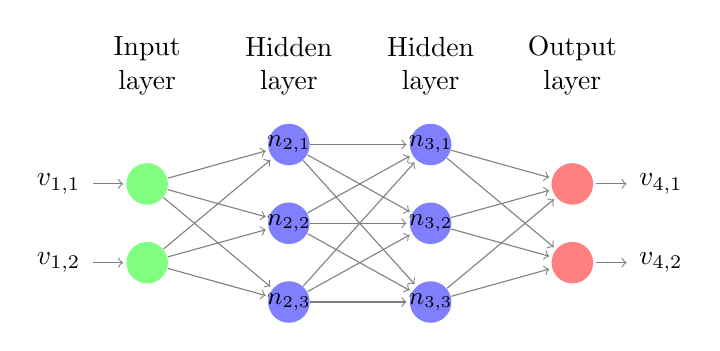
\begin{tikzpicture}[shorten >=1pt,->,draw=black!50, node distance=\layersep]
    \tikzstyle{every pin edge}=[<-,shorten <=1pt]
    \tikzstyle{neuron}=[circle,fill=black!25,minimum size=15pt,inner sep=0pt]
    \tikzstyle{input neuron}=[neuron, fill=green!50];
    \tikzstyle{output neuron}=[neuron, fill=red!50];
    \tikzstyle{hidden neuron}=[neuron, fill=blue!50];
    \tikzstyle{annot} = [text width=4em, text centered]

    % Draw the input layer nodes
    \foreach \name / \y in {1,...,2}
    % This is the same as writing \foreach \name / \y in {1/1,2/2,3/3,4/4}
        \node[input neuron, pin=left:$v_{1,\y}$] (I-\name) at (0,-\y) {};
        %\node[input neuron, pin=left:Input \#\y] (I-\name) at (0,-\y) {};

    % Draw the 1st hidden layer nodes
    \foreach \name / \y in {1,...,3}
        \path[yshift=0.5cm]
            node[hidden neuron] (H1-\name) at (\layersep,-\y cm) {};

    % Draw the 2nd hidden layer nodes
    \foreach \name / \y in {1,...,3}
        \path[yshift=0.5cm]
            node[hidden neuron] (H2-\name) at (\layersep*2,-\y cm) {};

    % Draw the output layer node
    \node[output neuron,pin={[pin edge={->}]right:$v_{4,1}$}, right of=H2-2, yshift=0.5cm] (O1) {};
    \node[output neuron,pin={[pin edge={->}]right:$v_{4,2}$}, right of=H2-2, yshift=-0.5cm] (O2) {};

    % Connect every node in the input layer with every node in the
    % hidden layer.
    \foreach \source in {1,...,2}
        \foreach \dest in {1,...,3}
            \path (I-\source) edge (H1-\dest);

    \foreach \source in {1,...,3}
        \foreach \dest in {1,...,3}
            \path (H1-\source) edge (H2-\dest);

    \foreach \source in {1,...,3}
         \path (H2-\source) edge (O1);

    \foreach \source in {1,...,3}
         \path (H2-\source) edge (O2);

    % Annotate the layers
    \node[annot,above of=H1-1, node distance=1cm] (hl1) {Hidden layer};
    \node[annot,above of=H2-1, node distance=1cm] (hl2) {Hidden layer};
    \node[annot,left of=hl1] {Input layer};
    \node[annot,right of=hl2] {Output layer};

    \node[annot, right of=H1-1, node distance=0.0cm] (hl1) {\small $n_{2,1}$};
    \node[annot, right of=H1-2, node distance=0.0cm] (hl1) {\small $n_{2,2}$};
    \node[annot, right of=H1-3, node distance=0.0cm] (hl1) {\small $n_{2,3}$};
    \node[annot, right of=H2-1, node distance=0.0cm] (hl1) {\small $n_{3,1}$};
    \node[annot, right of=H2-2, node distance=0.0cm] (hl1) {\small $n_{3,2}$};
    \node[annot, right of=H2-3, node distance=0.0cm] (hl1) {\small $n_{3,3}$};
\end{tikzpicture}
}
  \caption{A simple neural network}
  \label{fig:nn}
\end{figure}
